% --- [ Hammock Method ] -------------------------------------------------------

\subsection{Hammock Method}
\label{sec:hammock_method}

The Hammock method is a control flow analysis method which identifies control flow primitives in CFGs based on subgraph isomorphisms. More specifically, a set of high-level control flow primitives may be represented as canonical single-entry single-exit subgraphs\footnote{\textit{One potential reference for the naming of the Hammock method, is that the subgraphs are single-entry single-exist and are thus connected in two end-points, analogous to hammocks.}} (see figure \ref{fig:graph_representations}), and these subgraphs may be identified in CFGs using subgraph isomorphism search algorithms \cite{node_splitting}.

\begin{savenotes}
	\begin{figure}[htbp]
		\centering
		% if
		\begin{subfigure}[ht]{0.23\textwidth}
			\centering
			\begin{subfigure}[ht]{0.45\textwidth}
				\lstinputlisting[language=go, style=go, breaklines=false, numbers=none]{inc/primitives/if.c}
			\end{subfigure}
			\begin{subfigure}[ht]{0.42\textwidth}
				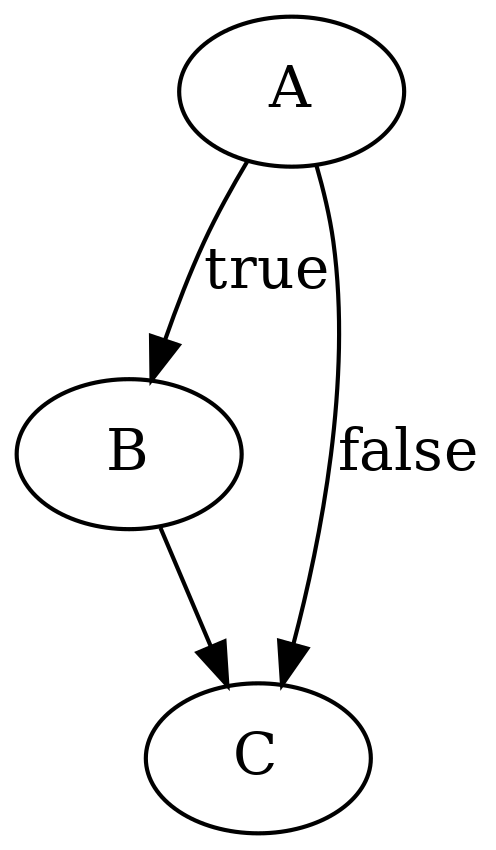
\includegraphics[width=\textwidth]{inc/primitives/if.png}
			\end{subfigure}
			\caption{1-way conditional; entry: \texttt{A}, exit: \texttt{C}.}
			\label{fig:if_graph_representation}
		\end{subfigure}
		\qquad
		% if_else
		\begin{subfigure}[ht]{0.28\textwidth}
			\centering
			\begin{subfigure}[ht]{0.45\textwidth}
				\lstinputlisting[language=go, style=go, breaklines=false, numbers=none]{inc/primitives/if_else.c}
			\end{subfigure}
			\begin{subfigure}[ht]{0.50\textwidth}
				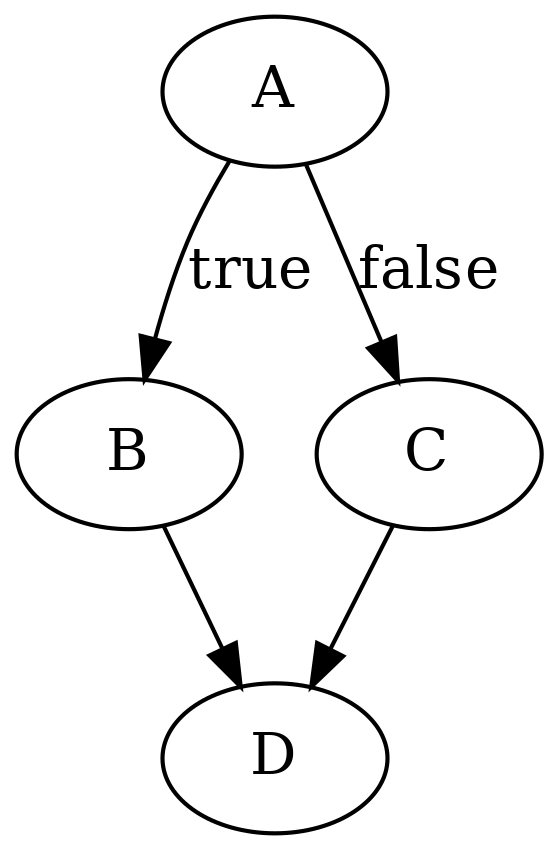
\includegraphics[width=\textwidth]{inc/primitives/if_else.png}
			\end{subfigure}
			\caption{2-way conditional; entry: \texttt{A}, exit: \texttt{D}.}
			\label{fig:if_else_graph_representation}
		\end{subfigure}
		\qquad
		% if_return
		\begin{subfigure}[ht]{0.30\textwidth}
			\centering
			\begin{subfigure}[ht]{0.45\textwidth}
				\lstinputlisting[language=go, style=go, breaklines=false, numbers=none]{inc/primitives/if_return.c}
			\end{subfigure}
			\begin{subfigure}[ht]{0.50\textwidth}
				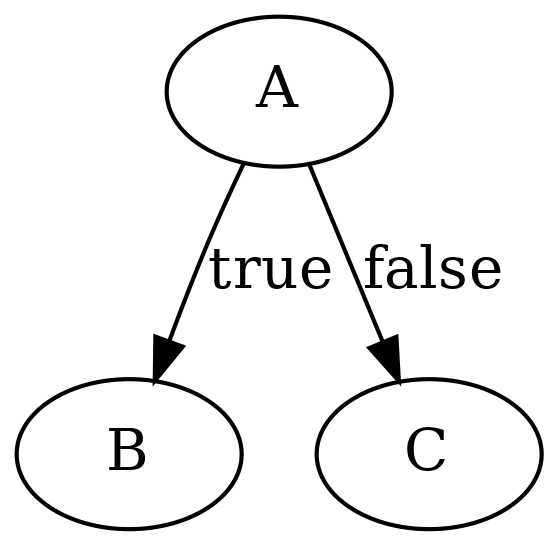
\includegraphics[width=\textwidth]{inc/primitives/if_return.png}
			\end{subfigure}
			\caption{1-way condition with return statement in body; entry: \texttt{A}, exit: \texttt{C}.}
			\label{fig:if_return_graph_representation}
		\end{subfigure}
		\qquad
		% pre_loop
		\begin{subfigure}[ht]{0.32\textwidth}
			\centering
			\begin{subfigure}[ht]{0.45\textwidth}
				\lstinputlisting[language=C, style=go, breaklines=false, numbers=none]{inc/primitives/pre_loop.c}
			\end{subfigure}
			\begin{subfigure}[ht]{0.50\textwidth}
				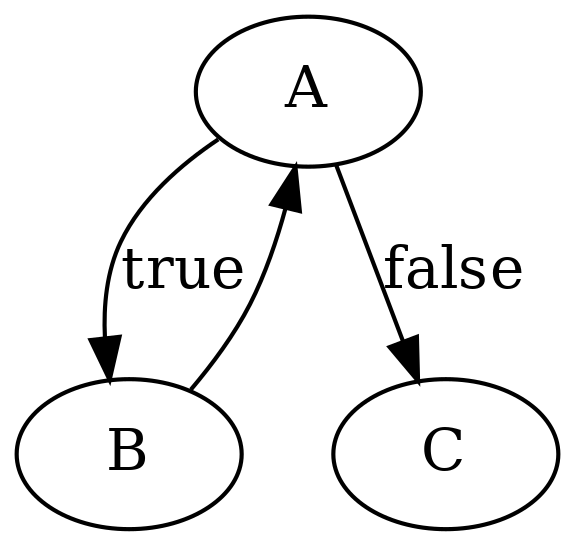
\includegraphics[width=\textwidth]{inc/primitives/pre_loop.png}
			\end{subfigure}
			\caption{pre-test loop; entry: \texttt{A}, exit: \texttt{C}.}
			\label{fig:pre_loop_graph_representation}
		\end{subfigure}
		\qquad
		% post_loop
		\begin{subfigure}[ht]{0.30\textwidth}
			\centering
			\begin{subfigure}[ht]{0.50\textwidth}
				\lstinputlisting[language=C, style=go, breaklines=false, numbers=none]{inc/primitives/post_loop.c}
			\end{subfigure}
			\begin{subfigure}[ht]{0.35\textwidth}
				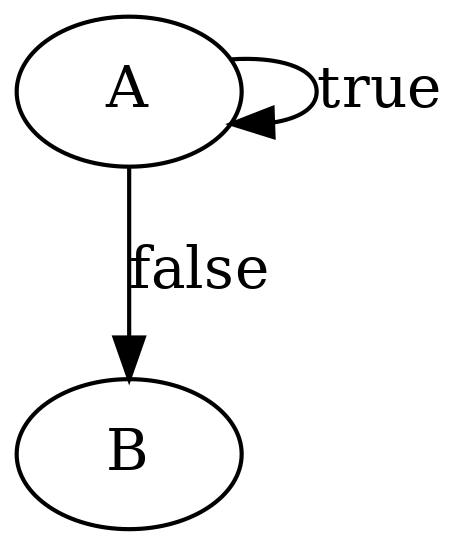
\includegraphics[width=\textwidth]{inc/primitives/post_loop.png}
			\end{subfigure}
			\caption{post-test loop; entry: \texttt{A}, exit: \texttt{B}.}
			\label{fig:post_loop_graph_representation}
		\end{subfigure}
		\qquad
		% seq
		\begin{subfigure}[ht]{0.24\textwidth}
			\centering
			\begin{subfigure}[ht]{0.20\textwidth}
				\lstinputlisting[language=C, style=go, breaklines=false, numbers=none]{inc/primitives/seq.c}
			\end{subfigure}
			\begin{subfigure}[ht]{0.35\textwidth}
				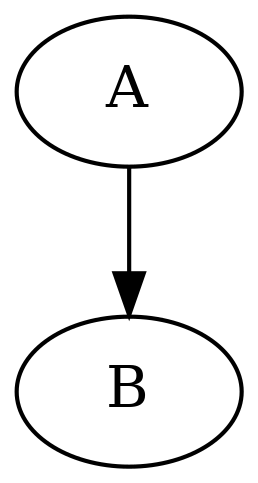
\includegraphics[width=\textwidth]{inc/primitives/seq.png}
			\end{subfigure}
			\caption{consecutive statements; entry: \texttt{A}, exit: \texttt{B}.}
			\label{fig:seq_graph_representation}
		\end{subfigure}
		\caption{The pseudo-code and graph representation of various high-level control flow primitives with denoted entry and exit nodes.\protect\footnote{Note, the Hammock method section is in part adapted from section 2.2.3 (Control Flow Analysis) of \cite{compositional_decompilation}, as written by the same author as this project.}}
		\label{fig:graph_representations}
	\end{figure}
\end{savenotes}

% TODO: rephrase the following paragraph.

To recover nested control flow primitives, the Hammock method iteratively performs subgraph isomorphism search to locate canonical subgraphs of high-level control flow primitives; and once a subgraph has been located, merges the nodes of the subgraph into a single node, which has the incoming edges of the entry node and the outgoing edges of the exit node; as illustrated in figure \ref{fig:subgraph_merge}. This process is repeated until the CFG either contains a single node or no more subgraph isomorphisms can be located, in which case high-level control flow primitives corresponding to of the CFG were fully or partially recovered, respectively.

\begin{figure}[htbp]
	\centering
	\begin{subfigure}[ht]{0.17\textwidth}
		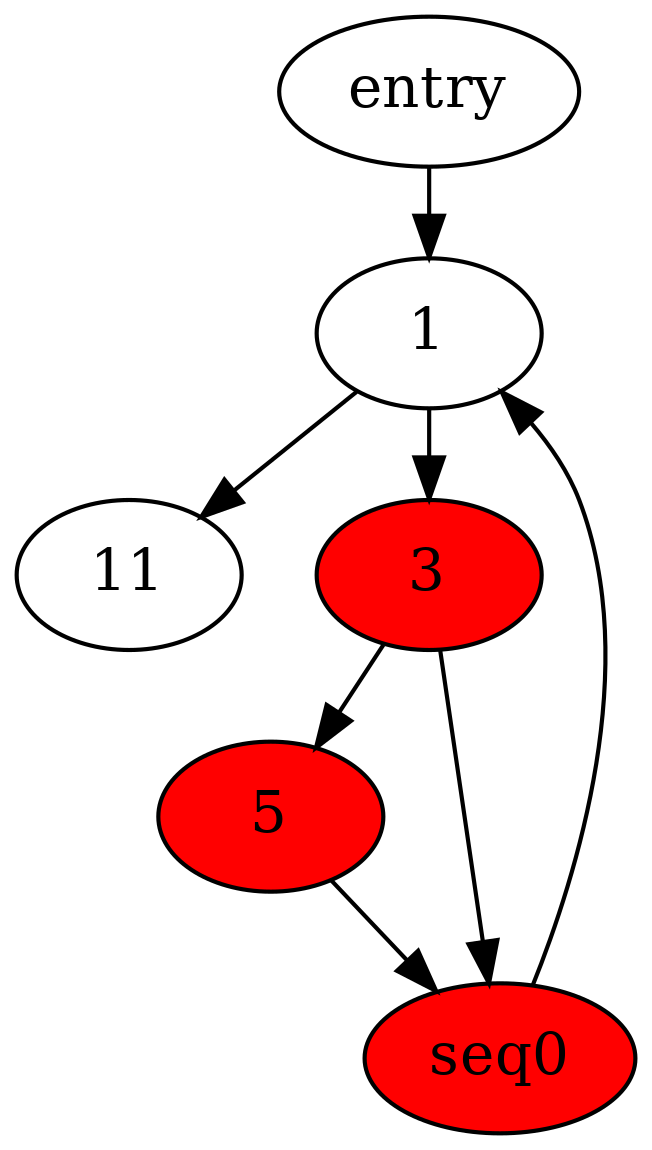
\includegraphics[width=\textwidth]{inc/3_background/cfg_pre_merge.png}
	\end{subfigure}
	\qquad
	\begin{subfigure}[ht]{0.17\textwidth}
		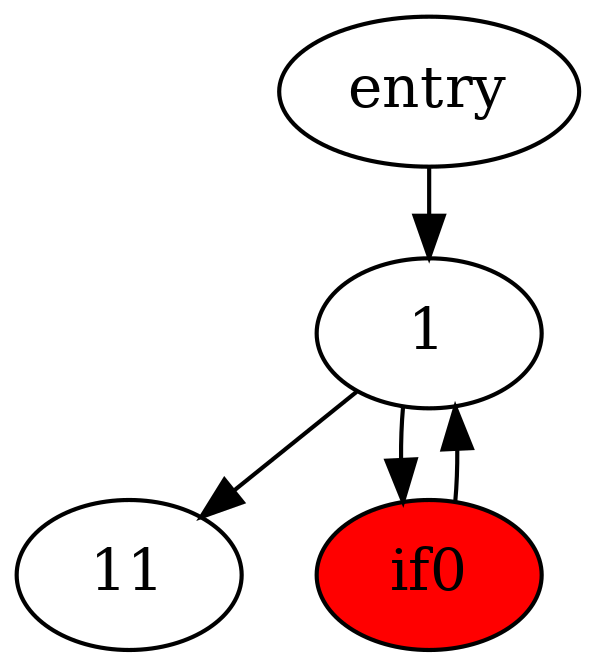
\includegraphics[width=\textwidth]{inc/3_background/cfg_post_merge.png}
	\end{subfigure}
	\caption{The left side illustrates the CFG of a function in which the graph representation of a 1-way conditional (see figure~\ref{fig:if_graph_representation}) has been identified, and the right side illustrates the same CFG after the subgraph has been replaced with a single node (i.e. \texttt{if0}) that inherits the predecessors of the subgraph entry node (i.e. \texttt{3}) and the successors of the subgraph exit node (i.e. \texttt{seq0}).}
	\label{fig:subgraph_merge}
\end{figure}
